\documentclass[13pt]{article}

\usepackage{graphicx}
\usepackage{booktabs}
\usepackage{multirow}
\usepackage{amsmath}
\usepackage{color}

\usepackage{fontspec}
\setmainfont{Arial}

\usepackage[paperwidth=174mm, paperheight=62.5mm, margin=0cm]{geometry}
% \renewcommand{\familydefault}{\sfdefault}
\usepackage{fontspec}
\setmainfont{Arial}
\setlength{\parindent}{0pt}

\begin{document}
\begin{tabular}{c@{\hspace{5mm}}l}
  \multicolumn{1}{l}{\large{A}}&\large{C}\\
  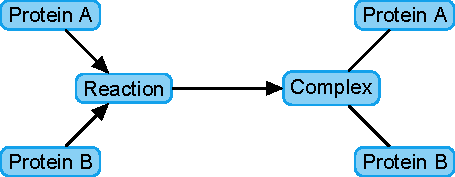
\includegraphics[scale=0.85]{Figure3a.pdf}&\multirow{4}{*}[7em]{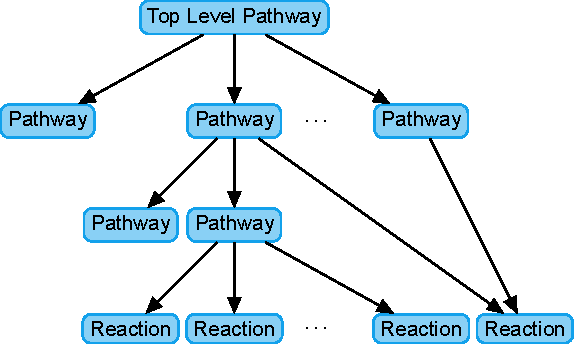
\includegraphics{Figure3c.pdf}}\\
  \\
  \multicolumn{1}{l}{\large{B}}&\\
  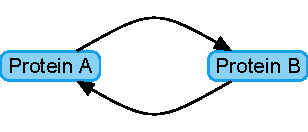
\includegraphics[scale=0.85]{Figure3b.pdf}&\\
\end{tabular}

\end{document}

